\documentclass[a4paper, 12pt]{book}
\usepackage[english]{babel}
%\usepackage{mathpazo}
% page layout
\usepackage[left=20mm, right=20mm, top=25mm]{geometry}
\geometry{a4paper}

% appendices
\usepackage[toc,page]{appendix}

% images
\usepackage{graphicx}

% colored headings
\usepackage{xcolor}

% equation numbering
\usepackage{amsmath}
\makeatletter
\def\tagform@#1{\maketag@@@{\ignorespaces\sffamily(#1)\unskip\@@italiccorr}}
\makeatother

% bookmarks
\usepackage{bookmark}

% dedication
\newenvironment{dedication}
{\clearpage             % new page
 \thispagestyle{empty}  % no header and footer
 \vspace*{\stretch{1}}  % top space
 %\itshape               % italics text
 \raggedleft            % flush to the right margin
}
{\par                   % end paragraph
 \vspace{\stretch{3}}   % bottom space (3x top space)
 \clearpage             % finish page
}

% sectioning
\usepackage{titlesec}

% titleformat{name}
% {title style}
% {number style}
% {space between number and title}
% {before-title code}

\titleformat{\part}[display]
  {\normalfont \sffamily \bfseries \centering}
  {\color{red!70!black} \Large \partname \, \thepart}
  {10pt} % vertical spacing
  {\Huge}

\titleformat{\chapter}[display]
  {\normalfont \sffamily \bfseries}
  {\color{red!70!black} \large \chaptertitlename \, \thechapter}
  {1pt}
  {\titlerule[1pt] \vspace{7pt} \Huge}

\titleformat{\section}
  {\normalfont \sffamily \Large}
  {\color{blue!70!black} §\bfseries\thesection}
  {10pt}
  {\bfseries}

\titleformat{\subsection}
  {\normalfont \sffamily \large}
  {\color{blue!70!black} §\bfseries\thesubsection}
  {10pt}
  {\bfseries}

\titleformat{\subsubsection}
  {\normalfont \sffamily}
  {\color{red!70!black} §\bfseries\thesubsubsection}
  {10pt}
  {\bfseries}

\renewcommand{\appendixtocname}{\sffamily Appendices}
\renewcommand{\appendixpagename}{\sffamily \Huge \bfseries Appendices}

% custom table of contents
\usepackage{tocloft}

\renewcommand{\cfttoctitlefont}{\sffamily \Huge \bfseries} % title font
% part
\renewcommand{\cftpartfont}{\sffamily \large \bfseries}
\renewcommand{\cftpartpagefont}{\sffamily \large \bfseries}
\renewcommand{\cftpartpresnum}{\sffamily \color{red!70!black}}
% chapter
\renewcommand{\cftchapfont}{\sffamily \bfseries}
\renewcommand{\cftchappagefont}{\sffamily \bfseries}
\renewcommand{\cftchappresnum}{\sffamily \color{red!70!black}}
% section
\renewcommand{\cftsecfont}{\sffamily}
\renewcommand{\cftsecpagefont}{\sffamily}
\renewcommand{\cftsecpresnum}{\sffamily \color{blue!70!black}}
% subsection
\renewcommand{\cftsubsecfont}{\sffamily}
\renewcommand{\cftsubsecpagefont}{\sffamily}
\renewcommand{\cftsubsecpresnum}{\sffamily \color{blue!70!black}}

% unnumbered chapter
\titleformat{name = \chapter, numberless}[block]
  {\centering \sffamily \bfseries \Large}
  {}
  {0pt}
  {}

% headers and foooters
\usepackage{fancyhdr}
\setlength{\headheight}{15pt}

% part name
\let\Oldpart\part
\newcommand{\parttitle}{}
\renewcommand{\part}[1]{\Oldpart{#1}\renewcommand{\parttitle}{#1}}

% no random page numbers
\fancypagestyle{plain}{%
  \fancyhf{} % clear all header and footer fields
  \renewcommand{\headrulewidth}{0pt}
  \renewcommand{\footrulewidth}{0pt}
}

% custom headers and footers
\renewcommand{\chaptermark}[1]{\markboth{#1}{#1}}
\pagestyle{fancy}
\fancyhead{}
\fancyfoot{}

\fancypagestyle{body}{%
  \fancyhead[LE,RO]{\sffamily\thepage}%
  \fancyhead[LO]{\sffamily \color{blue!70!black}\chaptername\ \thechapter\color{black} :\ \leftmark}%
  \fancyhead[RE]{\sffamily \color{blue!70!black}\partname\ \thepart\color{black} :\ \parttitle}%
}

% special header for Introduction
\fancypagestyle{introd}{%
  \fancyhead[LE,RO]{\sffamily \thepage}%
  \fancyhead[RE,LO]{\sffamily \leftmark}%
}

% special header for Contents
\fancypagestyle{contents}{%
  \fancyhead[LE,RO]{\sffamily \thepage}%
  \fancyhead[RE,LO]{\sffamily }%
}

% special header for Appendix
\fancypagestyle{append}{%
  \fancyhead[LE,RO]{\sffamily \thepage}%
  \fancyhead[LO]{\sffamily \color{blue!70!black}\appendixname\ \thechapter \color{black}:\ \leftmark}%
  \fancyhead[RE]{\sffamily Appendices}%
}

% special header for Bibliography
\fancypagestyle{biblio}{%
  \fancyhead[LE,RO]{\sffamily \thepage}%
  \fancyhead[RE,LO]{\sffamily Bibliography}%
}

% no blank pages
\let\cleardoublepage\clearpage
% removes indentation
\setlength{\parindent}{0pt}
% add subsubsection numbering
\setcounter{secnumdepth}{3}

% math
\usepackage{amsmath}
\usepackage{amssymb}
\usepackage{amsfonts}
\usepackage{amsthm}
\usepackage{mathtools}
\usepackage{mathrsfs}
%\usepackage{tensor}

% physics
\usepackage{braket}

% chemistry
\usepackage{chemformula}

% footnotes
\usepackage{footnote}

% bold text

\newcommand{\bctxt}[1]{\textcolor{blue!70!black}{\textbf{#1}}}

\newcommand{\bcdef}[1]{\textcolor{green!35!black}{\textbf{#1}}}

\newcommand{\bcth}[1]{\textcolor{red!35!black}{\textbf{#1}}}

\newcommand{\bclemma}[1]{\textcolor{blue!35!black}{\textbf{#1}}}

\newcommand{\bcprop}[1]{\textcolor{cyan!35!black}{\textbf{#1}}}

\newcommand{\bcex}[1]{\textcolor{yellow!35!black}{\textbf{#1}}}

% fancy environments
\usepackage[many]{tcolorbox}
\BeforeBeginEnvironment{tcolorbox}{\savenotes}
\AfterEndEnvironment{tcolorbox}{\spewnotes}

\tcbuselibrary{theorems}

\NewTcbTheorem[number within=section]{definition}{Definition}{%
  enhanced,%
  breakable,%
  colback = green!5,%
  colframe = green!5,%
  coltitle = green!35!black,%
  fonttitle = \sffamily\bfseries,%
  sharp corners,%
  boxrule = 0pt,%
  detach title,%
  before upper = {\tcbtitle\\[4pt]},%
  left = 5pt,%
  right = 5pt,%
  top = 5pt,%
  bottom = 5pt,%
  separator sign none,%
  description delimiters parenthesis,%
  description font = \mdseries%
}{def}

\newtcbtheorem[number within=section]{theorem}{Theorem}{%
  enhanced,%
  breakable,%
  colback = red!5,%
  colframe = red!5,%
  coltitle = red!35!black,%
  fonttitle = \sffamily\bfseries,%
  sharp corners,%
  boxrule = 0pt,%
  detach title,%
  before upper = {\tcbtitle\\[4pt]},%
  left = 5pt,%
  right = 5pt,%
  top = 5pt,%
  bottom = 5pt,%
  separator sign none,%
  description delimiters parenthesis,%
  description font = \mdseries%
}{th}

\newtcbtheorem[number within=tcb@cnt@theorem]{corollary}{Corollary}{%
  enhanced,%
  breakable,%
  colback = red!5,%
  colframe = red!5,%
  coltitle = red!35!black,%
  fonttitle = \sffamily\bfseries,%
  sharp corners,%
  boxrule = 0pt,%
  detach title,%
  before upper = {\tcbtitle\\[4pt]},%
  left = 5pt,%
  right = 5pt,%
  top = 5pt,%
  bottom = 5pt,%
  separator sign none,%
  description delimiters parenthesis,%
  description font = \mdseries%
}{cor}

\newtcbtheorem[number within=section]{lemma}{Lemma}{%
  enhanced,%
  breakable,%
  colback = blue!5,%
  colframe = blue!5,%
  coltitle = blue!35!black,%
  fonttitle = \sffamily\bfseries,%
  sharp corners,%
  boxrule = 0pt,%
  detach title,%
  before upper = {\tcbtitle\\[4pt]},%
  left = 5pt,%
  right = 5pt,%
  top = 5pt,%
  bottom = 5pt,%
  separator sign none,%
  description delimiters parenthesis,%
  description font = \mdseries%
}{lemma}

\newtcbtheorem[number within=lemma]{lemcorollary}{Corollary}{%
  enhanced,%
  breakable,%
  colback = blue!5,%
  colframe = blue!5,%
  coltitle = blue!35!black,%
  fonttitle = \sffamily\bfseries,%
  sharp corners,%
  boxrule = 0pt,%
  detach title,%
  before upper = {\tcbtitle\\[4pt]},%
  left = 5pt,%
  right = 5pt,%
  top = 5pt,%
  bottom = 5pt,%
  separator sign none,%
  description delimiters parenthesis,%
  description font = \mdseries%
}{cor}

\newtcbtheorem[number within=section]{proposition}{Proposition}{%
  enhanced,%
  breakable,%
  colback = cyan!5,%
  colframe = cyan!5,%
  coltitle = cyan!35!black,%
  fonttitle = \sffamily\bfseries,%
  sharp corners,%
  boxrule = 0pt,%
  detach title,%
  before upper = {\tcbtitle\\[4pt]},%
  left = 5pt,%
  right = 5pt,%
  top = 5pt,%
  bottom = 5pt,%
  separator sign none,%
  description delimiters parenthesis,%
  description font = \mdseries%
}{prop}

\newtcbtheorem[number within=proposition]{propcorollary}{Corollary}{%
  enhanced,%
  breakable,%
  colback = cyan!5,%
  colframe = cyan!5,%
  coltitle = cyan!35!black,%
  fonttitle = \sffamily\bfseries,%
  sharp corners,%
  boxrule = 0pt,%
  detach title,%
  before upper = {\tcbtitle\\[4pt]},%
  left = 5pt,%
  right = 5pt,%
  top = 5pt,%
  bottom = 5pt,%
  separator sign none,%
  description delimiters parenthesis,%
  description font = \mdseries%
}{cor}

\newtcbtheorem[number within=section]{example}{Example}{%
  enhanced,%
  breakable,%
  colback = yellow!10,%
  colframe = yellow!5,%
  coltitle = yellow!35!black,%
  fonttitle = \sffamily\bfseries,%
  sharp corners,%
  boxrule = 0pt,%
  detach title,%
  before upper = {\tcbtitle\\[4pt]},%
  left = 5pt,%
  right = 5pt,%
  top = 5pt,%
  bottom = 5pt,%
  separator sign none,%
  description delimiters parenthesis,%
  description font = \mdseries%
}{ex}

\newtcolorbox{proofbox}{%
  enhanced,%
  breakable,%
  colback = black!5,%
  colframe = black!5,%
  sharp corners,%
  boxrule = 0pt,%
  left = 5pt,%
  right = 5pt,%
  top = 5pt,%
  bottom = 5pt,%
  borderline west = {1pt}{0pt}{black!70},%
}

% custom references
\newcommand{\eref}[1]{\textsf{Eq.\,\ref{#1}}}
\newcommand{\eeref}[2]{\textsf{Eq.\,\ref{#1}-\ref{#2}}}
\newcommand{\dref}[1]{\textsf{Def.\,\ref{#1}}}
\newcommand{\ddref}[2]{\textsf{Def.\,\ref{#1}-\ref{#2}}}
\newcommand{\tref}[1]{\textsf{Th.\,\ref{#1}}}
\newcommand{\pref}[1]{\textsf{Prop.\,\ref{#1}}}
\newcommand{\lref}[1]{\textsf{Lemma\,\ref{#1}}}
\newcommand{\exref}[1]{\textsf{Ex.\,\ref{#1}}}

\newcommand{\secref}[1]{\textcolor{red!70!black}{\textsf{§\ref{#1}}}}

% hyper-references
\usepackage{hyperref}
\hypersetup{
  colorlinks = true,
  urlcolor = cyan,
  % linkcolor defined directly in \toc environment
  citecolor = green!70!black,
}

\newcommand{\toc}{%
  \hypersetup{linkcolor = black}%
  \tableofcontents%
  \hypersetup{linkcolor = red!70!black}%
}

% extended integral symbols
\usepackage{esint}

% text
\newcommand{\virgolette}[1]{``\text{#1}"}
\newcommand{\tildetext}{\raise.17ex\hbox{$\scriptstyle\mathtt{\sim}$}}

% greek
\newcommand{\Chi}{\text{X}}

% custom math symbols
\newcommand{\abs}[1]{\left\lvert#1\right\rvert}
\newcommand{\norm}[1]{\left\lVert#1\right\rVert}
\newcommand{\sgn}[1]{\mathrm{sgn}\,#1}
\newcommand{\pa}{\partial}
\newcommand{\na}{\nabla}
\newcommand{\tens}[1]{\mathrm{#1}}
\newcommand{\defeq}{\mathrel{\vcenter{\baselineskip0.5ex \lineskiplimit0pt
                     \hbox{\scriptsize.}\hbox{\scriptsize.}}}%
                     =}
\newcommand{\eqdef}{=%
                     \mathrel{\vcenter{\baselineskip0.5ex \lineskiplimit0pt
                     \hbox{\scriptsize.}\hbox{\scriptsize.}}}}
\newcommand{\ve}[1]{\mathbf{#1}}
\newcommand{\hilb}{\mathscr{H}}
\newcommand{\fock}{\mathscr{F}}
\DeclareMathOperator{\diag}{diag}
\newcommand{\sqg}{\sqrt{\tens{g}}}
\newcommand{\sqgm}{\sqrt{-\tens{g}}}
\newcommand{\cm}{\mathcal{C}^{\infty}(\mathcal{M})}
\DeclareMathOperator{\lspan}{span}
\newcommand{\xm}{\mathfrak{X}(\mathcal{M})}
\DeclareMathOperator{\id}{id}
\newcommand{\ld}{\mathcal{L}}
\newcommand{\lm}[1]{\Lambda^{#1}(\mathcal{M})}
\newcommand{\hrm}[1]{\mathrm{Harm}^{#1}(\mathcal{M})}
\DeclareMathOperator{\ran}{ran}
\DeclareMathOperator{\tr}{tr}
\DeclareMathOperator{\Tr}{Tr}
\DeclareMathOperator{\End}{End}
\DeclareMathOperator{\im}{Im}
\newcommand{\dd}{\mathrm{d}}
\newcommand{\bs}[1]{\boldsymbol{#1}}
\newcommand{\dg}{^\dagger}
\DeclareMathOperator{\Aut}{Aut}
\DeclareMathOperator{\ad}{ad}
\DeclareMathOperator{\Ad}{Ad}
\newcommand{\lag}{\mathcal{L}}
\newcommand{\ham}{\mathcal{H}}
\newcommand{\act}{\mathcal{S}}
\newcommand{\normord}{\mathfrak{N}}
\newcommand{\tempord}{\mathfrak{T}}
\newcommand{\parity}{\mathcal{P}}
\newcommand{\chargec}{\mathcal{C}}
\newcommand{\timer}{\mathcal{T}}
\newcommand{\covder}{D}
\newcommand{\mat}{\mathcal{M}}
\newcommand{\smo}{\mathcal{O}}
\newcommand{\msb}{\overline{\text{MS}}}

\newcommand{\grad}{\boldsymbol{\nabla}}
\newcommand{\dive}{\boldsymbol{\nabla}\cdot}
\newcommand{\rot}{\boldsymbol{\nabla}\times}
\newcommand{\lap}{\triangle}

% small \overleftrightarrow
\makeatletter
\newcommand{\overleftrightsmallarrow}{\mathpalette{\overarrowsmall@\leftrightarrowfill@}}
\newcommand{\overrightsmallarrow}{\mathpalette{\overarrowsmall@\rightarrowfill@}}
\newcommand{\overleftsmallarrow}{\mathpalette{\overarrowsmall@\leftarrowfill@}}
\newcommand{\overarrowsmall@}[3]{%
  \vbox{%
    \ialign{%
      ##\crcr
      #1{\smaller@style{#2}}\crcr
      \noalign{\nointerlineskip}%
      $\m@th\hfil#2#3\hfil$\crcr
    }%
  }%
}
\def\smaller@style#1{%
  \ifx#1\displaystyle\scriptstyle\else
    \ifx#1\textstyle\scriptstyle\else
      \scriptscriptstyle
    \fi
  \fi
}
\makeatother
\newcommand{\smlra}[1]{\overleftrightsmallarrow{#1}}
\newcommand{\smla}[1]{\overleftsmallarrow{#1}}
\newcommand{\smra}[1]{\overrightsmallarrow{#1}}

% functions
\DeclareMathOperator{\sech}{sech}
\DeclareMathOperator{\Exp}{Exp}

% number sets
\newcommand{\N}{\mathbb{N}}
\newcommand{\Z}{\mathbb{Z}}
\newcommand{\Q}{\mathbb{Q}}
\newcommand{\R}{\mathbb{R}}
\newcommand{\C}{\mathbb{C}}
\newcommand{\K}{\mathbb{K}}

% groups
\newcommand{\Ot}{\mathrm{O}(3)}
\newcommand{\SOt}{\mathrm{SO}(3)}
\newcommand{\On}[1]{\mathrm{O}(#1)}
\newcommand{\SOn}[1]{\mathrm{SO}(#1)}
\newcommand{\Un}[1]{\mathrm{U}(#1)}
\newcommand{\SUn}[1]{\mathrm{SU}(#1)}
\newcommand{\GL}[1]{\mathrm{GL}(#1)}
\newcommand{\SL}[1]{\mathrm{SL}(#1)}

% units of measure
\newcommand{\m}{\,\mathrm{m}}
\newcommand{\ang}{\,\mathrm{\AA}}
\newcommand{\fm}{\,\mathrm{fm}}

\newcommand{\barn}{\,\mathrm{barn}}

\newcommand{\cels}{\,^{\circ}\mathrm{C}}

\newcommand{\ev}{\,\mathrm{eV}}
\newcommand{\kev}{\,\mathrm{keV}}
\newcommand{\mev}{\,\mathrm{MeV}}
\newcommand{\gev}{\,\mathrm{GeV}}
\newcommand{\tev}{\,\mathrm{TeV}}

% particles
\newcommand{\g}{\mathrm{g}}
\newcommand{\w}{\mathrm{W}}
\newcommand{\z}{\mathrm{Z}}

% custom title page
\newcommand{\customtitlepage}[7]{%
  \begin{titlepage}
    \centering
    % department logo at the top of the page
    
\includegraphics[width=0.75\textwidth]{imgs/unimi.jpg}\\
    \vspace{1cm} % ddjust the vertical space as needed
    {\large Bachelor's Degree in #1 \par} % degree title
    \vspace{1cm}
    %\hrule % horizontal line
    \vspace{1cm} % adjust the vertical space as needed
    {\large \sffamily \textbf{#2} \par} % thesis title (bold)
    \vspace{9cm} % adjust the vertical space as needed
    
    \begin{minipage}[H]{\textwidth}
      \small Supervisor: \\
      \normalsize #3 \\
      \vspace{1cm}
    \end{minipage}
    \begin{minipage}[t]{\textwidth}
      \raggedleft
      \small Student: \\
      \normalsize #4\\ % student name
      \normalsize Matr.: #5 % student number
    \end{minipage}

    % academic year section at the bottom of the page
    \vspace{\fill}
    {\normalsize Academic Year #6 \par}
    
  \end{titlepage}
}

\usepackage[font=small]{caption}
\newcommand{\um}{\mathfrak{m}}

\usepackage{overarrows}
\usepackage{slashed}
\usepackage{simpler-wick}

\usepackage{tikz}
\usepackage[compat=1.1.0]{tikz-feynman}


% bibliography

\usepackage{csquotes}
\usepackage[
backend = biber,
style = numeric-comp,
sorting = ynt
]{biblatex}
\addbibresource{bibl.bib}

\renewbibmacro{in:}{}

\AtEveryBibitem{%
	\clearfield{publisher}%
	\clearfield{month}%
	\clearfield{numpages}%
	\clearfield{issue}%
	\clearfield{isbn}%
}

\DeclareFieldFormat[book,article]{journaltitle}{#1}
\DeclareFieldFormat[book,article]{volume}{\mkbibbold{#1}}


\title{Thesis}
\author{Lucrezia Bioni}

\begin{document}

\frontmatter

\customtitlepage{Physics}{Next-to-Leading Order QCD Corrections to Scattering Processes Using $\theta$-Parameters in the Nested Soft-Collinear Subtraction Scheme}{Prof. Raoul Horst Röntsch}{Lucrezia Bioni}{13655A}{2024--2025}
\clearpage

\chapter*{Abstract}
\selectlanguage{english}
Perturbative Quantum Chromodynamics (QCD) corrections are essential for achieving high-precision theoretical predictions in particle physics, which makes them fundamental for interpreting data from modern particle accelerators, such as the Large Hadron Collider (LHC) at CERN. As experimental precision increases, theoretical predictions must also attain a level of accuracy that allows for meaningful comparisons with data. This requires extending perturbative calculations beyond the leading order (LO) to include next-to-leading order (NLO) and higher-order corrections in the strong coupling constant $\alpha_s$. These corrections account for crucial physical effects, such as real parton emissions and virtual loop contributions. \\
A significant challenge in calculating these higher-order corrections arises from the presence of infrared (IR) singularities, which occur when partons become soft or collinear. Although the sum of all contributions to a cross-section is finite, due to the cancellation of divergences between real emissions and virtual loops, each individual term is divergent. To manage these divergences and obtain finite, numerically stable results, it is necessary to introduce subtraction schemes that regularize the singularities locally in the phase space. \\
Over the past few decades, a variety of subtraction schemes have been developed for this purpose. Among them, the Nested Soft-Collinear (NSC) Subtraction Scheme has gained particular prominence due to its conceptual clarity, modular structure, and consistent extensibility from NLO to next-to-next-to-leading order (NNLO). The NSC scheme achieves a local cancellation of infrared singularities by factorizing soft and collinear limits in a nested manner. Furthermore, its modular nature allows the subtraction terms for complex processes to be built from a limited set of basic components, making it well-suited for implementation in automated Monte Carlo frameworks. \\
The aim of this thesis is to extend the NSC Subtraction Scheme by introducing a set of continuous parameters, called $\theta$-parameters, which systematically restrict the subtraction procedure to the singular, unresolved regions of phase space where soft and collinear singularities occur. Specifically, the parameter $\theta_s$ limits the energy of unresolved partons in the soft limit, while $\theta_i$ controls their angular separation in the collinear limit. The central motivation for this development is to improve numerical stability and efficiency in Monte Carlo integrations, particularly for multi-leg processes where redundant phase-space coverage can significantly slow down convergence. \\
The implementation and analytical study in this thesis demonstrate that introducing $\theta$-parameters preserves the theoretical consistency and modular nature of the NSC scheme. These parameters modify only the soft and collinear (real) contributions, while leaving the virtual corrections and those from PDF renormalization unchanged. Specifically, they appear in the $I_{\mathrm{S}}(\epsilon)$ and $I_{\mathrm{C}}(\epsilon)$ operators, which are part of the soft and collinear counterterms for the infrared-divergent scattering amplitudes. Crucially, the $\theta$-parameters do not compromise the cancellation of the infrared $1/\epsilon^2$ and $1/\epsilon$ poles when all contributions are summed. The coefficient of the $1/\epsilon^2$ pole in $I_{\mathrm{S}}(\epsilon)$ is independent of any parameter, and, while the coefficients of the $1/\epsilon$ poles in $I_{\mathrm{S}}(\epsilon)$ and $I_{\mathrm{C}}(\epsilon)$ depend on $\theta_s$, this dependence cancels out in their sum. This confirms that the modified NSC scheme yields the same physical cross-sections as the standard one. \\
Therefore, the study presented in this thesis contributes to the ongoing effort to improve the efficiency and reliability of higher-order QCD computations. Such improvements are fundamental to continue testing the Standard Model and searching for new Physics beyond its confines.


\newpage

\toc

\pagestyle{contents}

\mainmatter

\chapter{Introduction}

\section{The Standard Model}


As Aristotle stated, women and men began to philosophize due to wonder. From antiquity, a profound sense of astonishment towards the natural world has driven humans to investigate phenomenological reality. This drive is so profound and innate in humanity that – starting with the first philosophers, called ``Pre-Socratics"  or ``natural philosophers" – it led them to inquire into the nature of the ``archè" ($\acute{\alpha}\rho\chi\acute{\eta}$), the primordial principle and fundamental constituent underlying all of nature. This enduring pursuit of fundamental knowledge evolved through the centuries and, in the last one, culminated in the experimental discovery of a multitude of subatomic particles. Their proliferation was such that it prompted the noted physicist Enrico Fermi to remark: ``If I could remember the names of all these particles, I'd be a botanist". This apparent complexity, however, has been successfully resolved through the development of a robust theoretical framework that classifies these particles and describes their interactions via gauge theories: the Standard Model (SM). \\
The SM is formulated within the mathematical framework of Quantum Field Theory (QFT), which unifies the principles of Quantum Mechanics and Special Relativity to describe phenomena at high energies, or equivalently, subatomic scales. Its predictions have been rigorously tested and confirmed by experiments, most notably with the discovery of the Higgs boson in 2012.  Despite its success, there are significant efforts to discover Physics beyond the SM. This is driven not only by the natural attempt at falsification that should be applied to every scientific theory, but also by several phenomena that the model cannot explain. These include the existence of dark matter and dark energy, the observed matter-antimatter asymmetry, and the origin of neutrino masses \cite{Campbell:2017}. \\

\section{Collider physics}
One of the principal methods of research in high-energy physics is collider physics \cite{ellis}. Using colliders, it is possible to artificially accelerate particles and to reach extremely high center-of-mass energy. Operating at the energy frontier is crucial: higher-energy collisions enable events with greater momentum transfer and energy deposition. These events are essential because concentrating significant energy within a tiny volume allows us to excite new, heavy elementary particles from the vacuum, and study their properties. Experiments at the energy frontier are conducted at the Large Hadron Collider (LHC) at CERN: in a 27-kilometer ring, proton beams collide at a center-of-mass energy of approximately 13.6 TeV. Although these energy scales have allowed us to study the known fundamental interactions – with the exception of gravity – in great detail, they have not been sufficient for the discovery of new particles.  Since increasing the energy of the colliding particles is not feasible with existing technology, the focus of collider experiments in the next decade will shift towards higher experimental precision. This precision is crucial for refining our understanding of the Standard Model (SM), especially the properties of the Higgs boson: in fact, it is the agent of electroweak (EW) symmetry breaking, which is a fundamental component of the theory. Moreover, precision measurements serve as a powerful probe for new physics, which may reveal itself as subtle deviations from SM predictions in processes involving only known particles.  However, testing the Standard Model with experimental results necessitates reliable theoretical predictions for hadron collider processes.

\section{QCD and hard scattering processes}
A theoretical description of hadron collisions is complicated primarily by our limited knowledge of the strong force, which binds the elementary constituents of hadrons. Strong interactions are described by Quantum Chromodynamics (QCD), a non-Abelian gauge theory based on the SU(3) symmetry group. The QCD Lagrangian is not analytically solvable, making it extremely difficult to understand proton dynamics from first principles. A way to overcome these obstacles becomes manifest when we consider how hadrons collide at high energies \cite{Asteriadis2020}. Typically, they undergo either elastic scattering or diffractive dissociation: in the first case, they collide but remain intact; in the second, they disintegrate into a small number of hadrons. However, on rare occasions, a more interesting phenomenon can occur: the elementary partons that compose the hadrons can interact and exchange a large amount of momentum ($\sim 100 \,\text{GeV}$). This is the case in so-called ``hard scattering processes," which are central to probing the electroweak scale, the Higgs boson, and potential new physics. Their importance is directly related to a key feature of the strong force: asymptotic freedom. The essence of this property is the weakening of the colour force at short distances \cite{ellis}. In this high-energy regime, the interacting partons can be approximated as being nearly free, which permits a perturbative description of the strong interaction. The strength of these interactions is governed by the coupling constant $\alpha_{\text{S}}$. Due to asymptotic freedom, $\alpha_{\text{S}}$ is on the order of $0.1$ at energies relevant for contemporary colliders\footnote{This value is energy-dependent; $\alpha_{\text{S}}\sim0.1$ is typical at energies around 100 GeV.}. This makes the strong force about ten times stronger than the electromagnetic interaction (whose coupling constant is $\alpha\sim1/137$), yet sufficiently small to allow for the application of well-defined perturbative approximation methods.

\section{Hadronic cross-section and factorization theorem}
A framework for describing these short-distance hard scattering processes is provided by the collinear factorization theorem \cite{Collins:1987pm}. Within this framework, colliding hadrons are treated as beams of partons, each carrying a certain fraction of the hadron's total momentum. The probability of finding a parton with a specific energy fraction is encoded in the Parton Distribution Functions (PDFs). These functions are universal, meaning they are independent of the specific scattering process being studied. Consequently, PDFs can be measured in one set of experiments and then used to make predictions for many others \cite{Melnikov2018}. The short-distance interaction of partons produces final states composed of Standard Model particles, such as leptons, gauge bosons, and additional QCD partons. The final-state partons, which are the direct products of the perturbative calculation, cannot be observed directly due to confinement\footnote{Quark confinement is the phenomenon that prevents quarks and gluons from propagating as free particles over macroscopic distances.}. Instead, they evolve into collimated sprays of hadrons \cite{Salam:2010nqg}. We interpret these partons as the seeds of hadronic jets and define the resulting sprays as jets themselves. At high energies, the properties of these jets are largely determined by the perturbative dynamics of their initiating parton and are only mildly affected by non-perturbative QCD effects. \\
The asymptotic freedom of QCD is what enables a perturbative description of the strong interaction. However, it is crucial to recognize that the precise mechanism allowing us to decouple the motion of partons from the proton's dynamics is the separation of energy scales involved. Interactions in the Standard Model typically probe energy scales on the order of $Q \sim 100  \, \text{GeV} - 1 \, \text{TeV}$, while the characteristic energy scale of hadronic structure and confinement is significantly lower, $\Lambda_{\text{QCD}} \sim 100 \, \text{MeV}$. \\
The production cross section for final states involving QCD jets and other Standard Model particles in hard hadronic collisions is thus given by
\begin{equation}
    \text{d}\sigma = \sum_{a, b} \int_0^1 \text{d}x_1 \text{d}x_2 \, f_{a}(x_1, \mu_\text{F}) \, f_{b}(x_2,\mu_\text{F}) \, \text{d}\hat \sigma_{a,b}(x_1,x_2,\mu_\text{F},\mu_\text{R};\mathcal{O}) \, \left(1+ \mathcal{O}\left(\frac{\Lambda_{\text{QCD}}}{Q} \right)^n \right), \qquad n\geq1
    \label{fact-theor}
\end{equation}
where $f_{a,b}$ are the parton distribution functions mentioned above; $a, b \in \{g, d/\bar{d}, u/\bar{u}, s/\bar{s}, c/\bar{c}, b/\bar{b} \}$  represent the types of partons (gluons or quarks) inside the two colliding hadrons; $x_1, x_2$ are respectively the momentum fractions carried by partons $a$ and $b$; and $\mathcal{O}$ is an infrared-finite observable. \\
The non-perturbative corrections in Eq. \ref{fact-theor} are suppressed by powers of the ratio $\Lambda_{\text{QCD}}/Q$: in this case, $Q$ represents the hard scale of the process, typically identified as the lowest transverse momentum ($p_T$) cut applied to final-state partons. For a typical cut of $Q \sim 20\ \text{GeV}$, this ratio is of order $10^{-2}$. The exact power $n$ of this suppression is process-dependent, and not always immediately evident, though for many applications the leading power is $n = 2$. This implies that the theoretical uncertainty from factorizing non-perturbative physics is of order $\mathcal{O}(10^{-4})$. Even when the leading power is only $n = 1$, the non-perturbative effects would be at the percent level ($\sim 10^{-2}$). This is comparable in size to the Next-to-Next-to-Leading Order (NNLO) QCD corrections for many processes. Therefore, a precise description of a process requires the inclusion of at least NNLO perturbative corrections before the inherent uncertainty from power corrections becomes significant.\\
This formalism establishes a clear distinction between the short-distance perturbative process and the long-distance non-perturbative physics. The boundary between these two regimes is defined by the factorization scale ($\mu_\text{F}$). Processes with a momentum transfer $Q > \mu_\text{F}$ are treated as the hard scatter of point-like partons, calculable within perturbation theory. Physics at scales $Q < \mu_\text{F}$, which describes how the partons are bound within the proton, is incorporated into the non-perturbative Parton Distribution Functions (PDFs). \\
The other scale present in the factorized cross-section in Eq. \ref{fact-theor} is the renormalization scale ($\mu_\text{R}$). Its necessity arises because the calculation of partonic interactions in QCD using Feynman diagrams often results in ultraviolet (UV) divergences. These infinities do not indicate a fundamental error in the theory, but suggest a distinction between the bare parameters in the Lagrangian and physically observable quantities. The process of renormalization allows us to absorb these divergences into a redefinition of the Lagrangian's parameters, providing finite expressions for measurable quantities. The consequence of this procedure is that the coupling constant becomes a function of the energy scale, a phenomenon known as ``running" \cite{ellis}. The renormalization scale $\mu_\text{R}$ is the energy at which the coupling constant is defined, thereby encapsulating the quantum corrections of the theory. \\
Throughout this thesis, we set $\mu_\text{F} = \mu_\text{R} = \mu$. While a physical prediction must be independent of these arbitrary scales, cross-sections calculated within a fixed-order perturbative expansion exhibit a dependence on both the renormalization and factorization scales. Therefore, varying the scales around a central value and observing how the prediction changes provides a standard method for estimating the uncertainty associated with the truncation of the perturbative series. \\

\begin{figure}[!ht]
	\centering
	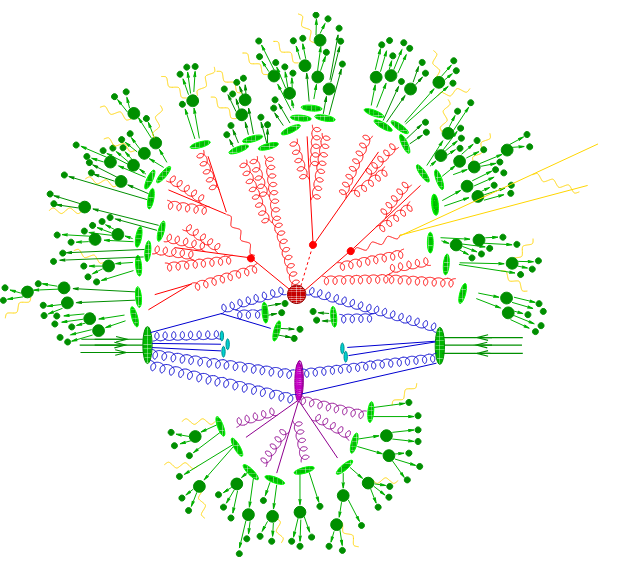
\includegraphics[width=0.7\textwidth]{imgs/hadron-collision.png}
	\caption{Sktetch of an hard hadron-hadron collision at a collider like the LHC. The central red blob represents the hard interaction, a high-energy collision between two partons, calculable using perturbative QCD. The incoming and outgoing partons emit initial-state (blue) and final-state (red) radiation, producing many secondary particles. Softer underlying event activity (purple) arises from additional partonic interactions within the protons. A key feature is the hierarchy of energy scales: the hard process occurs at high energies ($Q>\Lambda_{\text{QCD}}$), while subsequent radiation and hadronization (green) take place at progressively lower scales, eventually transitioning to non-perturbative physics around $\Lambda_{\text{QCD}}$. Figure from \cite{Hoeche:2014}.}
	\label{hadron-collision}
\end{figure}

Referring to Eq. \ref{fact-theor}, we can state that only the left-hand side represents a physically measurable quantity. The right-hand side, in contrast, consists of unobservable components: the parton distribution functions (PDFs), which are extracted from experimental data, and the partonic cross-section $\mathrm{d}\hat{\sigma}_{a,b}$, which is calculable within perturbation theory. It is therefore essential to understand how this latter quantity is computed.


\section{Partonic cross-section}
We consider the inclusive\footnote{The inclusive cross-section counts every collision event that creates a specific particle, whether it appears alone, with jets, or with any other additional radiation. It gives the total production rate, ignoring the details of what else is produced alongside it.} production of $N$ jets at a hadron collider, together with a color-neutral system $X$
\begin{equation}
    pp \rightarrow X + N \, \mathrm{jets}  \, .
\end{equation}
As discussed above, we can use asymptotic freedom of QCD to expand the partonic cros section $\mathrm{d}\hat{\sigma}_{a,b}$ in Eq. \ref{fact-theor} in powers of the strong and the electroweak coupling constants, $\alpha_{\text{S}}$ and $\alpha$,
\begin{equation}
    \text{d} \hat{\sigma}_{a,b} = \text{d} \hat{\sigma}_{a,b}^{(0,0)} + \alpha_s \text{d} \hat{\sigma}_{a,b}^{(1,0)} + \alpha_s^2 \text{d} \hat{\sigma}_{a,b}^{(2,0)} + \alpha_s^3 \text{d} \hat{\sigma}_{a,b}^{(3,0)} + \alpha \text{d} \hat{\sigma}_{a,b}^{(0,1)} + \alpha \alpha_s \text{d} \hat{\sigma}_{a,b}^{(1,1)} + \dots .
\end{equation}
Due to the different values of the coupling constants, at the same order they have a different impact on the final result: at NLO, QCD corrections account for approximately $10\%$, while EW account for $1\%$; at NNLO, QCD corrections account for $1\%$. Throughout this thesis, we will focus on the calculation of NLO QCD corrections. \\
The first term in this expansion $\text{d} \hat{\sigma}_{a,b}^{(0,0)} \equiv \text{d} \hat{\sigma}_{a,b}^{\text{LO}}$ is called Leading Order (LO), and it is defined as \cite{Devoto:2025jql}
\begin{equation}
    2s_{a,b}\text{d} \hat{\sigma}_{a,b}^{\text{LO}} = \mathcal{N} \int \mathrm{d}\Phi (2\pi)^4 \mathrm{dLips}_X \delta^{(4)}(p_\mathcal{H_f}+p_X-p_a-p_b) \left|\mathcal{M}_0(p_a,p_b;p_{\mathcal{H}_f},p_X) \right|^2 \mathcal{O}(p_\mathcal{H},p_X).
    \label{leading-order}
\end{equation}
With $\mathcal{H}_f$, we denote the list of final-state resolved particles, and $p_{\mathcal{H}_f}$ is their momentum, while $p_X$ denotes the momentum of the color-singlet in the hard process. $\mathcal{N}$ is a normalization factor: it takes into account color and spin averages as well as symmetry factors. With $s_{a,b}$, we express the partonic center-of-mass energy squared: $s=(p_a+p_b)^2=2 p_a\cdot p_b$, considering massless partons. The matrix element for the considered process is denoted by $\mathcal{M}_0$, and $\mathcal{O}$ represents an infrared-safe observable that ensures the final state contains at least $N$ resolved jets. This latter feature is crucial because infrared dynamics are non-perturbative and, consequently, cannot be described by an expansion in $\alpha_\mathrm{s}$. Finally, $\mathrm{dLips}_X$ is the Lorentz-invariant phase space for the colorless particle $X$, including the momentum-conserving delta function, and $\mathrm{d}\Phi$ is the Lorentz-invariant phase space for the final-state particles.
\begin{equation}
    \mathrm{d}\Phi= \prod_{i \in \mathcal{H}_f} [\mathrm{d}p_i], \qquad [\mathrm{d}p_i]=\frac{\mathrm{d}^3p_i}{(2\pi)^32E_i},
\end{equation}
where $[\mathrm{d}p_i]$ is the phase-space element of a final-state parton $i$. Moreover, in Eq. \ref{leading-order}, summation over spins and colors of final-state partons, and averaging over spins and colors of initial-state partons are assumed.  \\
For notational compactness, we introduce the function $F^{ab}_{\mathrm{LM}}$, defined as in Section 2 of \cite{Devoto:2023rpv}
\begin{equation}
    F^{ab}_{\mathrm{LM}} = \mathrm{dLips}_X |\mathcal{M}_0|^2 \, \mathcal{O}.
    \label{flm}
\end{equation}
We denote the integration over the final-state phase space of Eq. \ref{flm} with the angular brackets $\langle\dots\rangle$, and obtain exactly Eq. \ref{leading-order}
\begin{equation}
    2s_{a,b} \, \text{d} \hat{\sigma}_{a,b}^{\text{LO}} = \langle F^{ab}_{\mathrm{LM}}[\dots] \rangle.
\end{equation} \\
At Leading Order (LO), calculations are performed directly. The tree-level matrix elements can be computed easily using helicity techniques and colour-subamplitude decompositions \cite{Altarelli:1977zs}, and are then integrated, either numerically or analytically. \\
The strong coupling constant in hard scattering processes is small enough to allow for a perturbative description, but not enough to make higher-order corrections entirely negligible. Therefore, in order to claim high precision, we also need to compute QCD corrections. According to the factorization theorem, the computed partonic cross-section should be insensitive to long-distance effects, which are absorbed into the parton distribution functions. The QCD corrections instead account for short-distance, high-energy effects at higher orders in the coupling constant. The NLO correction $\text{d} \hat{\sigma}_{a,b}^{(1,0)} \equiv \text{d} \hat{\sigma}_{a,b}^{\mathrm{NLO}} $ to a partonic cross section consists of three terms: the one-loop (virtual) contribution, the real emission contribution, and the contribution related to parton distribution functions


\begin{equation}
    \mathrm{d} \hat{\sigma}_{a,b}^{\mathrm{NLO}} = \mathrm{d} \hat{\sigma}_{a,b}^{\mathrm{V}} + \mathrm{d} \hat{\sigma}_{a,b}^{\mathrm{R}} + \mathrm{d} \hat{\sigma}_{a,b}^{\mathrm{pdf}}.
\end{equation} 

The last term, $\mathrm{d} \hat{\sigma}_{a,b}^{\mathrm{pdf}}$, is generated by the renormalization of the PDFs at LO, and its expression is known \cite{Catani:1996vz}. The other terms, $\mathrm{d} \hat{\sigma}_{a,b}^{\mathrm{V}}$ and $\mathrm{d} \hat{\sigma}_{a,b}^{\mathrm{R}}$, are related to either the emission of an additional leg in the Feynman diagram, i.e., an extra parton in the final state (real correction), or to the emission and reabsorption of a parton through a loop (virtual correction).  \par\bigskip
\begin{figure}[!ht]
	\centering
	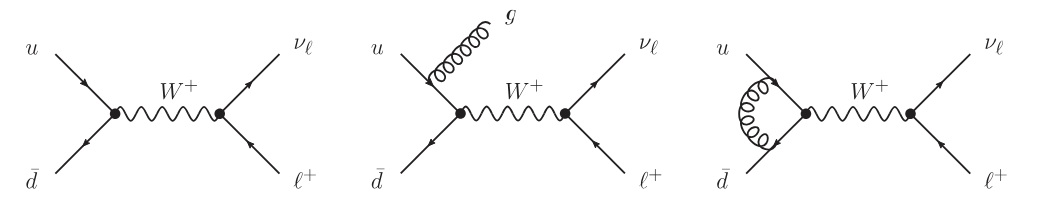
\includegraphics[width=0.9\textwidth]{imgs/real-and-virtual.png}
	\caption{Feynman diagrams for W boson production at hadron colliders. The diagram on the left corresponds to the leading-order (LO) calculation of the total cross-section. The diagrams shown in the middle and on the right represent the real and virtual corrections, respectively, which together constitute the next-to-leading-order (NLO) contributions to the total cross-section. Figure from \cite{Campbell:2017}}.
	\label{hadron-collision}
\end{figure}
It is important to emphasize that while the concepts of ``real" and ``virtual" radiation are physically well-defined, their separate contributions to the partonic cross-section, $\mathrm{d}\hat{\sigma}_{a,b}$, are not physically observable. The division into real and virtual terms is therefore a computational tool, introduced to organize the calculation and manage the various contributions more effectively. \\ The treatment of these terms is non-trivial, as they exhibit divergences in specific energy regimes. The virtual contributions, for instance, contain ultraviolet (UV) singularities. These are removed through the process of renormalization\footnote{Throughout this thesis, we work with UV-renormalized matrix elements.}, a procedure that ensures physical observables, when expressed in terms of appropriately defined renormalized parameters, become insensitive to the high-energy UV region. \\ Furthermore, the low-momentum (soft) and small-angle (collinear) kinematic regions produce singularities in both the real and virtual contributions. These infrared (IR) singularities are not independent: the real and virtual corrections are fundamentally linked by their infrared behavior. The divergence of scattering amplitudes in the soft or collinear limit means these kinematic configurations must be carefully handled to obtain meaningful results. Consequently, a precise procedure for removing these divergences is of the highest importance for calculating finite cross-sections.

\section{Infrared poles and their cancellation}
In order to deal with IR divergences, it is convenient to employ dimensional regularization \cite{THOOFT1973455}. This technique involves the analytical continuation of momentum space from $4$ to $d=4-2\epsilon$ dimensions, where $\epsilon \in \mathbb{C}$ and $\mathrm{Re}(\epsilon)<0$. In this framework, divergences appear as poles in $1/\epsilon$ in the complex dimensional plane. \\
The virtual corrections $\mathrm{d} \hat{\sigma}_{a,b}^{\mathrm{V}}$ contain explicit infrared and collinear poles, which are independent of the details of the hard matrix element \cite{Catani:1996vz}. In contrast, the real emission contribution $\mathrm{d} \hat{\sigma}_{a,b}^{\mathrm{R}}$ contains kinematic singularities that only become explicit $1/\epsilon$ poles upon integration over the phase space of the additional final-state parton. However, we must avoid a naive integration over the entire radiation phase space, as it would render the cross section inclusive rather than differential, discarding all information on the kinematics of the radiated parton. This information is often crucial since jet properties provide essential data for defining experimental signatures. \\
QCD amplitudes for real emission processes become singular in kinematic limits where the gluon becomes soft (low energy) or any parton (quark, antiquark, gluon) is emitted collinearly to another parton. In these limits, the propagator of the emitted particle approaches its on-shell condition, leading to divergent behavior. To show this, consider a diagram that describes an emission of a gluon ($\um$) off an external incoming quark ($i$) line 
\begin{equation*}
  \begin{tikzpicture}[baseline = (r.base)]
    \begin{feynman}[inline = (r.base)]
      \vertex (a);
      \vertex[right = 2.5cm of a, dot] (b) {};
      \vertex[right = 2.5cm of b, circle, draw, fill=lightgray,  minimum size = 1.2cm] (c) {};

      \vertex[above = 1cm of b] (d);
      \vertex[right = 1.5cm of d] (e);

      \vertex[below = 0.25cm of b] (r);

      \diagram* {
	    (a) -- [fermion, momentum' = \(p_i\)] (b),
	    (b) -- [fermion, momentum' = \(p_i - p_\um\)] (c),

	    (b) -- [gluon, momentum = \(p_\um\)] (e),
        };
    \end{feynman}
  \end{tikzpicture}
  \quad \sim \quad
  \frac{1}{(p_i - p_\um)^2} = \frac{1}{2 E_i E_\um \left( 1 - \cos \theta_{i \um} \right)} \quad
  \xrightarrow[E_\um, \theta_{i \um} \to 0 ]{} \quad \infty \,.
\end{equation*}
For massless partons ($|\mathbf{p}_i|=E_i, \, |\mathbf{p}_i|^2=0$), the amplitude exhibits a clear divergence in both the soft and collinear limits, that is when $E_\um$ or $\theta_{i \um} \to 0$.\\
It is important to consider the origin of these infinities. The presence of divergences is, in fact, a manifestation of long-distance effects: they signal that non-perturbative contributions are entering our perturbative calculation. This could be a problem, as we lack methods to treat non-perturbative QCD effects from first principles \cite{Melnikov2018}. Fortunately, once the $1/\epsilon$ poles are extracted from both the virtual and real corrections, their sum is guaranteed to be free of infrared divergences due to the Bloch-Nordsieck \cite{PhysRev.52.54} and Kinoshita-Lee-Nauenberg theorems. Therefore, perturbative QCD corrections remain insensitive to the details of infrared physics. \\
However, achieving the cancellation of the $1/\epsilon$ poles by simply summing the real and virtual corrections is not straightforward. This complication arises because the virtual corrections are defined in an $n$-particle phase space, whereas the real corrections inhabit an ($n+1$)-particle phase space. We might think that this problem could be avoided by integrating over the phase space. However, this approach would only yield a total cross-section, not a differential one, as stated above. This mismatch in the dimensionality of the integration domains, combined with the need to extract the implicit $1/\epsilon$ poles from the real-emission contributions, without performing the full integration, is precisely why dedicated subtraction schemes are required. \\
Over time, various methods have been developed to perform fully differential QCD computations for hadron collider processes, both at NLO and NNLO. Among the existing methods, in this thesis we will focus on the Nested Soft-Collinear (NSC) Subtraction Scheme \cite{Caola:2017dug}, which will be detailed in Chapter \ref{NSC-SS}. The numerical stability and computational efficiency of this method can, however, be further improved. A step forward in this direction will be presented in Chapter \ref{NSC-SS-parameters}; this represents the original contribution of this thesis. 







\clearpage

\chapter{NLO QCD corrections in the NSC Subtraction Scheme}
\label{NSC-SS}
The singular limits of NLO QCD amplitudes, as well as the methods for using them to compute NLO QCD cross sections, are well established \cite{Frixione:1995ms,Catani:1996vz}. Furthermore, all the singular limits of QCD amplitudes necessary for calculating NNLO QCD corrections have been known for approximately two decades. However, it took significant time to determine how to combine these NNLO limits with the ideas from the NLO Frixione-Kunszt-Signer (FKS) subtraction scheme \cite{Frixione:1995ms} to construct a valid subtraction method for NNLO computations. Among the numerous proposed methods, the Nested Soft-Collinear Subtraction Scheme (NSC SS), introduced in \cite{Caola:2017dug}, is particularly attractive, for reasons that will become clear throughout the following discussion. \\
This chapter provides an overview of the main results achieved. Since the objective of this thesis is to implement parameters that allow for greater control over the integrated phase-space region, and since these parameters appear only in the real corrections, we will focus exclusively on the latter. Moreover, the divergent parts of the virtual corrections can be isolated using Catani's representation of renormalized one-loop scattering amplitudes \cite{Catani:1998bh}. Although these methods have been implemented up to NNLO, this thesis will focus on the NLO case, as its relative simplicity offers a clearer understanding of how to implement the parameters.

\section{Properties of Soft and Collinear partons}
\label{properties}
The desired method necessitates the isolation of singularities in the real corrections without integrating over the momenta of any of the final-state particles, in order to keep the kinematics of all the final-state particles intact. There are two key insights that allow us to overcome this obstacle. The first one is related to the behaviour of NLO QCD amplitudes at soft and collinear limits. \\For a generic QCD amplitude $\mathcal{M}$ involving $n$ partons with four-momenta $p_1, p_2, \dots, p_n$ and an additional soft gluon with vanishing four-momentum $p_\um$, the squared amplitude factorizes into (i) the squared amplitude for the hard process without the gluon and (ii) an eikonal factor that depends only on the color charges and momenta of the hard partons and the momentum of the soft gluon ($p_\um$) \cite{Catani:1999ss}
\begin{equation}
    \lim_{E_\um \rightarrow 0}|\mathcal{M}(p_1, p_2, \dots, p_n; p_\um)|^2= - 4\pi \alpha_s \mu^{2\epsilon} \sum_{i,j=1}^n \mathcal{S}_{ij}(p_\um) \vec{T}_i \cdot \vec{T_j} |\mathcal{M}_0(p_1, p_2, \dots, p_n)|^2,
    \label{ampl-soft}
\end{equation}
where the general eikonal factor is
\begin{equation}
    \mathcal{S}_{ij}(p_\um) = \frac{p_i \cdot p_j}{(p_i \cdot p_\um)(p_j \cdot p_\um)}  \,, 
    %\sim \frac{1}{E_\um^2}
\end{equation}
and the square of the color charges are $\vec{T}_i^2= C_F$ if $i$ is a quark or an anti-quark, and $\vec{T}_i^2= C_A$ if i is a gluon. \\
Whereas, in the collinear limit, i.e., the limit where a gluon is emitted parallel to a quark, the amplitude-squared factorizes into (i) a splitting function, which describes the probability for the quark to radiate the gluon collinearly at a given energy, and (ii) the squared hard amplitude, which now depends on the resulting quark momentum after the emission
\begin{equation}
    \lim_{\theta_{i \um \rightarrow 0}}|\mathcal{M}(p_1, \dots, p_n; p_\um)|^2 \sim P_{f_{[i\um]}f_i} |\mathcal{M}_0(p_1, \dots, p_n)|^2  \,.
    %\sim \frac{1}{(p_i-p_\um)^2} \sim (1-\cos(\theta_{i\um}))^{-1}\sim \theta_{i\um}^{-2}.
    \label{ampl-coll}
\end{equation}
The unresolved parton $\um$ could also be a quark or an antiquark. However, the emission of a soft quark leads to a convergent integral; consequently, no divergences are associated with soft quark or antiquark emissions. Divergences do arise in the collinear limit, but, as in the gluon case, the amplitude factorizes into a hard process involving a parton with rescaled momentum and a corresponding splitting function. \\
Equations \ref{ampl-soft} and \ref{ampl-coll} show that the dependence on $p_\um$ lies only in the eikonal function, while $\mathcal{M}_0$ is independent of $p_\um$. This remark will be fundamental to construct properly a subtraction method. \\
The second important insight is that, in singular kinematic regions, real emissions are always unresolved, meaning they lack a distinct experimental signature. Consequently, we can safely integrate over the singular regions of their phase space without losing any physically observable information. \\

\section{Why a subtraction method}
Let us first present the core idea of the subtraction formalism. We consider the integral
\begin{equation}
    I = \int_0^1 \mathrm{d}x \, \frac{1}{x^{1+\epsilon}} F(x),
\end{equation}
where $F(x)$ is an arbitrary function regular at $x=0$. The integrand diverges at the lower limit, and this singularity is regulated by the parameter $\epsilon$, which ultimately produces a $1/\epsilon$ pole upon integration. We want to isolate this pole analitically, and define the integral in such a way that the limit $\epsilon \to 0$ can be taken safely. To achieve this, we write $F(x)=[F(x)-F(0)]+F(0)$
\begin{equation}
    I = \int _0^1 \mathrm{d}x \, \frac{1}{x^{1+\epsilon}} [F(x)-F(0)]+F(0)\int_0^1 \mathrm{d}x \, \frac{1}{x^{1+\epsilon}},
\end{equation}
and, performing the integration in the second term, we get
\begin{equation}
    I = \int_0^1 \frac{\mathrm{d}x}{x}[F(x)-F(0)] - \frac{1}{\epsilon}F(0) + \mathcal{O}(\epsilon).
    \label{extraction-poles}
\end{equation}
This equation demonstrates that we have successfully isolated the $1/\epsilon$ pole in $I$ and regulated the integrand. As a result, the $\epsilon \to 0$ limit can now be taken safely, leaving an integral that is regular at $x=0$ and can be evaluated numerically.\\
Now, suppose we have a function $\mathcal{S}$ that reproduces the leading singular behaviour of $F^{ab}_{\mathrm{LM}}$ (defined in Eq. \ref{flm}) in all soft and collinear limits, and that can be integrated in the $d$-dimensional phase space of the unresolved parton $\um$. We can then write the real-emission cross section as
\begin{equation}
    2s_{a,b} \mathrm{d} \hat{\sigma}_{a,b}^{\mathrm{R}} = \int [\mathrm{d}p_{\um}] F^{ab}_{\mathrm{LM}} = \int [\mathrm{d}p_{\um}] (F^{ab}_{\mathrm{LM}} - \mathcal{S}) + \int [\mathrm{d}p_{\um}] \mathcal{S}
    \label{subtraction-flm}
\end{equation}
where $[\mathrm{d}p_{\um}]$ is the $d$-dimensional phase-space measure for the emitted gluon, now also incorporating the theta function to enforce energy conservation
\begin{equation}
    [\mathrm{d}p_{\um}] = \frac{\mathrm{d}^{d-1}p_\um}{(2 \pi)^{d-1}2E_\um} \theta(E_{\mathrm{max}}-E_\um),
\end{equation}
and $E_{\mathrm{max}}$ is an arbitrary energy scale that must be at least as large as the maximum energy allowed by the momentum-conserving $\delta$-functions in Eq. \ref{leading-order}.\\
On the right-hand side of Eq. \ref{subtraction-flm}, the first term is integrable in four-dimensional phase space, since the leading singular behaviour of $F^{ab}_{\mathrm{LM}}$ is removed by the subtraction term $\mathcal{S}$. As this integration is performed numerically using Monte Carlo (MC) methods, it is clear that restricting the integration region to the minimal necessary volume is crucial for improving the efficiency of the computation. \\
The second term involves only the unresolved parton $\um$, making it possible to integrate over its phase space without affecting the jet observables. Furthermore, as showed in Eq. \ref{extraction-poles}, this integration enables the extraction of $1/\epsilon$ poles, which describe the singular behaviour of $\mathcal{S}$ and, consequently, of the amplitude itself. Moreover, it resolves the problem of the dimensional mismatch between the integration domains of the virtual and real corrections. Thus, the cancellation of the poles with those arising from the virtual contributions becomes possible.

\section{Soft and Collinear operators}
Different subtraction schemes are characterized by different forms for $\mathcal{S}$, or, equivalently, $F(0)$. The FKS subtraction scheme, which constitutes the basis for the NSC method, constructs $\mathcal{S}$ directly from the soft and collinear limits. The efficacy of this approach becomes clear if we consider the behaviour of the amplitudes in these limits, as detailed in Section \ref{properties}: in both the soft and collinear cases, the amplitude squared factorizes into a  lower-multiplicity function $F^{ab}_{\mathrm{LM}}$, which is independent of the unresolved parton $\um$, and a singular term, whose integration over the phase space of parton $\um$ gives the explicit pole. Therefore, we introduce two operators that perform soft and collinear projections
\begin{equation}
    S_i A = \lim_{E_i \to 0} A \, , \qquad C_{ij}A = \lim_{\rho_{ij}\to 0}A \, ,
\end{equation}
where $\rho_{ij}= 1 - \vec{n}_i \cdot \vec{n}_j = 1 - \cos{\theta_{ij}}$, with $\vec{n}_i$ a unit vector that describes the direction of the momentum of the $i$-th particle in ($d-1$)-dimensional space, and $\theta_{ij}$ the angle between partons $i$ and $j$. These operators apply to all terms that follow them. \\
Thus, we identify $\mathcal{S}$ as the action of the soft and/or collinear operators on $F^{ab}_{\mathrm{LM}}$. As these operators capture the leading asymptotic behaviour of the product of the matrix element squared, the observable, and the phase space – namely, the definition of $F^{ab}_{\mathrm{LM}}$ in Eq. \ref{flm}, if this quantity is, instead, integrable, the operator acts as an annihilator. \\
The singularities are isolated and extracted sequentially, in a nested manner: first, we remove the soft singularities, and then the collinear and soft-collinear ones.

\section{Damping factors}
Paragrafo su Damping factors: come si gestisce lo spazio delle fasi \\
Ha senso inserirli per processi più generali.


\section{Different channels}
One of the most interesting features of the NSC subtraction scheme is that the subtractions for a generic process, complicated as much as we want, are built starting from a relatively small set of basic ingredients. In particular, for a process with ant number of partons or jest, we can split them up, and evaluate each contribution: what matters is only if we have two initials, two finals or one initial and one final partons which can become unresolved. These three different possibilities have been studied, respectively, in \cite{Caola:1902}, \cite{Caola:1907}, and \cite{Asteriadis:1910}.


La potenza di NSC SS sta nel fatto che the subtractions for a generic process are built from a relatively small set of basic ingredients. Paragrafo sui vari possibili canali, sul fatto che si possa descrivere un processo estremamente complesso sommando i vari contributi: conta solo se si abbia two initials (1902), two finals (1907) or one initial and one final (1910): illustro questi processi. (fare disegnetto con somma dei processi) \\
\section{Soft limit}
Paragrafo su soft singularities, e che forma hanno i contributi nei 3 processi considerati. \\
\section{Collinear limit}
Paragrafo su collinear singularities \\
\section{Soft-collinear limit}
Paragrafo su soft-collinear singularities \\
\section{Cancellation of poles}
è possibile dimostrare la cancellazione dei poli $1/\epsilon$ analiticamente e derivare i finite remainders. Non metto dimostrazione esplicita della cancellazione (sarebbe una ripetizione), ma cerco di spiegare la logica. 

\section{Draft}

\clearpage

\chapter{NLO QCD corrections with $\theta$-parameters in the NSC Subtraction Scheme}
\label{NSC-SS-parameters}

Il lavoro esposto nel capitolo precedente può essere ulteriormente generalizzato, come è stato fatto nei paper \cite{Devoto:2023rpv,Devoto:2025kin}. In questo capitolo ripercorriamo tali risultati, implementando theta parameters. Lo facciamo perché uno dei principali difetti di NSC SS è che la sua efficienza è un po' impattata dalla numerical integration of the subtraction terms.

\section{Damping factors}
Quando ho tanti partoni nel final state, introduco damping factor per identificare quello unresolved. Vedere 2310, pagine 6-8.

\section{Draft}

\clearpage

\bookmarksetupnext{level = -1}
\begin{appendices}
\pagestyle{append}

\chapter{Draft appendix}

\section{Draft}

Lorem ipsum dolor sit amet \cite{pauli}.

\clearpage
\end{appendices}

\bookmarksetupnext{level = -1}
\pagestyle{biblio}
\printbibliography[heading = bibintoc, title = {Bibliography}]

\end{document}